\section{Accuracy issues}

Achieving accurate image rectification is influenced by several factors. 
Here, we identify key challenges and strategies for improving accuracy:
\begin{enumerate} 
    \item \textit{Noise and numerical errors}: noise and numerical errors in the input data can significantly impact the rectification process, leading to inaccuracies. 
        Preprocessing techniques, such as noise filtering and data normalization, are essential to mitigate these issues and improve stability in the rectification calculations.
    \item \textit{Insufficient line information}: selecting appropriate lines to determine vanishing points is critical. Lines that are too close to each other may result in poorly defined vanishing points, introducing inaccuracies into the rectification. 
        It is important to select lines that are sufficiently spaced to ensure precise vanishing point estimation.
    \item \textit{Vanishing points near infinity}: when a vanishing point is nearly at infinity, achieving accurate affine rectification becomes challenging. 
        To address this issue, consider the following approaches:
        \begin{itemize}
            \item Draw two lines in the scene perpendicular to the original lines in the image. 
            If these lines are not parallel, adjust their intersections to make them parallel.
            This adjustment helps bring the vanishing point closer, making it easier to compute an affine transformation.
            \begin{figure}[H]
                \centering
                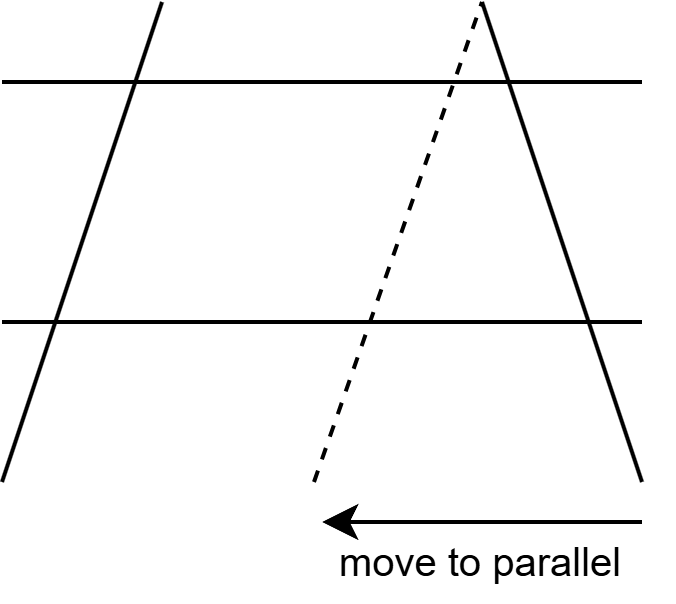
\includegraphics[width=0.3\linewidth]{images/vpi.png}
                \caption{Aligning lines to bring the vanishing point closer}
            \end{figure}
            After adjusting, apply affine reconstruction to obtain more accurate results.
            \begin{figure}[H]
                \centering
                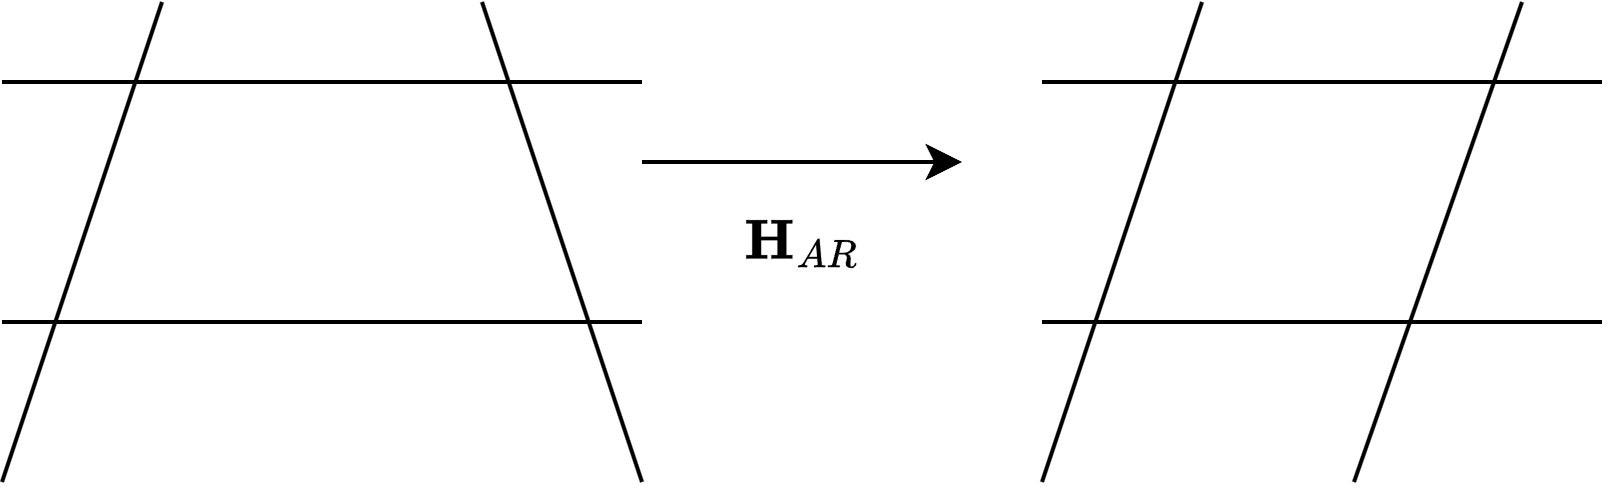
\includegraphics[width=0.3\linewidth]{images/ar.png}
                \caption{Applying affine reconstruction}
            \end{figure}
            \item For scenes with multiple sets of parallel lines, select one line from each set and randomly choose an additional pair of perpendicular lines. 
            Using these four lines, compute the matrix product $\mathbf{KK}^T$, where $\mathbf{K}$ represents the camera calibration matrix. 
            Derive $\mathbf{K}$ through Cholesky factorization and use it in the rectifying transformation:
            \[\mathbf{H}_{\text{rect}} = \begin{bmatrix} \mathbf{K} & \mathbf{t} \\ 0 & 1 \end{bmatrix}^{-1} \]
            where $\mathbf{t}$ is a translation vector. 
            This transformation corrects perspective distortions.
        \end{itemize}        
\end{enumerate}
The accuracy of image rectification is crucial for various computer vision and image processing applications, and addressing these issues is essential for obtaining reliable results.